\documentclass[11pt,a4paper]{article}

\usepackage[utf8]{inputenc}
\usepackage{graphicx}
\usepackage[spanish]{babel}
\usepackage{float}				%Para poner las imagenes exactamente donde se me cante las pelotas en caso de quererlo, poniendole [H]
\usepackage{amsmath}
\usepackage{epstopdf}
\usepackage{geometry}
\usepackage{hieroglf}
\usepackage{subcaption}
\usepackage[justification=centering]{caption}
\usepackage[colorinlistoftodos]{todonotes}
\usepackage[colorlinks=true, allcolors=blue]{hyperref}
\geometry{
a4paper,
left=20mm,
right=20mm,
top=25mm,
bottom = 20mm
}
\usepackage{float}
\usepackage{units}
% \usepackage{hyperref}   %Esto es para ir a los links

\newcommand{\rojo}[1]{\textcolor{red}{#1}}    % Comando para escribir texto en rojo




\title{\textbf{Matemática de los Sistemas Biológicos \\ Práctica 4}}

\author{
{F. M. Cabrera}
%[1ex] \small{\textit{ Facultad de Ciencias Exactas y Naturales.}} \\
%\small{\textit{Universidad de Buenos Aires. Ciudad Universitaria. Pabellón I. Buenos Aires. Argentina}}
}
\date{\textit{\today}}


% Esto modifica el interlineado
\renewcommand{\baselinestretch}{1}

\graphicspath{{Figuras/}}

\begin{document}

\maketitle

%\thispagestyle{empty} 


\setcounter{page}{1}

%\begin{abstract}


%\end{abstract}
%\vspace*{1cm}

Todo el código implementado en esta practica puede encontrarse \href{https://github.com/cabre94/MSB_IB}{acá}.


\section*{Ejercicio 1 - Modelo de Goodwin}

Tenemos un mecanismo de regulación de la expresión de un gen, descripto por
\begin{align}
    \frac{dm}{dt} &= \alpha_m g_{R}\left(p\right) - \beta_m m \\
    \frac{de}{dt} &= \alpha_e m - \beta_e e \\
    \frac{dp}{dt} &= \alpha_p e - \beta_p p
\end{align}
donde $m$ es la concentración del mRNA, que produce la enzima $e$, la cual contribuye a la producción de una proteína $p$. La regulación está controlada por la proteína, con una función de represión de la forma:
\begin{equation}
    g_R \left(p\right) = \frac{a}{b+cp^{h}}.
    \label{eq:represion}
\end{equation}

En la Fig. \ref{ej1:concentraciones_barrido_h} se observan los resultados de la simulación numérica realizada para distintos valores del parámetro de Hill $h$, fijando los valores del resto de los parámetros a $\alpha_m = \alpha_e = \alpha_e =1$, $a=b=c=1$ y $\beta_m = \beta_e = \beta_p = 0.1$. Luego de un periodo transitorio, se observa que para $h=8$ y $h=12$ las oscilaciones son sostenidas, con una mayor amplitud para $h=12$, mientras que para $h=6$ las oscilaciones son amortiguadas y terminan desapareciendo.

\begin{figure}[htb!]
    \centering
    \begin{subfigure}[b]{0.42\textwidth}
        \includegraphics[width=\textwidth]{../ej1_Resultados/h=6_Concentraciones.pdf}
    \end{subfigure}
    \begin{subfigure}[b]{0.42\textwidth}
        \includegraphics[width=\textwidth]{../ej1_Resultados/h=8_Concentraciones.pdf}
    \end{subfigure}
    \begin{subfigure}[b]{0.42\textwidth}
        \includegraphics[width=\textwidth]{../ej1_Resultados/h=12_Concentraciones.pdf}
    \end{subfigure}
    \caption{Evolución de las concentraciones de mRNA, proteína y enzima para distintos valores del parámetro de Hill $h$. Luego de un periodo transitorio, se observa que para $h=8$ y $h=12$ las oscilaciones son sostenidas, con una mayor amplitud para $h=12$, mientras que para $h=6$ las oscilaciones son amortiguadas y terminan desapareciendo.}
    \label{ej1:concentraciones_barrido_h}
\end{figure}

En la Fig. \ref{ej1:concentraciones_barrido_h_estacionario} se observan los mismos resultados que en la Fig. \ref{ej1:concentraciones_barrido_h} pero para tiempos mas largos, de manera de observar en detalle el periodo estacionario del sistema. Se observa que para $h=7$ las oscilaciones continúan disminuyendo su amplitud, al igual que para $h=8$ (aunque puede suceder que aun no se haya alcanzado el estado estacionario), pero para $h=10$ y $h=14$ las oscilaciones ya son sostenidas.

\begin{figure}[htb!]
    \centering
    \begin{subfigure}[b]{0.42\textwidth}
        \includegraphics[width=\textwidth]{../ej1_Resultados/m_estacionario.pdf}
    \end{subfigure}
    \begin{subfigure}[b]{0.42\textwidth}
        \includegraphics[width=\textwidth]{../ej1_Resultados/p_estacionario.pdf}
    \end{subfigure}
    \begin{subfigure}[b]{0.42\textwidth}
        \includegraphics[width=\textwidth]{../ej1_Resultados/e_estacionario.pdf}
    \end{subfigure}
    \caption{Estado estacionario de las concentraciones de mRNA, proteína y enzima para distintos valores del parámetro de Hill $h$. Se observa que para $h=7$ las oscilaciones continúan disminuyendo su amplitud, al igual que para $h=8$ (aunque puede suceder que aun no se haya alcanzado el estado estacionario), pero para $h=10$ y $h=14$ las oscilaciones ya son sostenidas.}
    \label{ej1:concentraciones_barrido_h_estacionario}
\end{figure}

Luego, utilizando un valor de $h=10$ en el cual se observaran oscilaciones, se busco estudiar el efecto en la dinámica del sistema al aumentar la degradación $\beta$ de las distintas concentraciones. El resto de parámetros $\alpha_i$ y $a$, $b$ y $c$ se mantuvieron iguales y se utilizo el mismo valor de la degradación tanto para el mRNA, la proteína y la enzima. En la Fig. \ref{ej1:concentraciones_barrido_b} se observan los resultados obtenidos para valores de $\beta$ iguales a $0.1$, $0.5$ y $1$. Al aumentar el valor de $\beta$ a $0.5$, primero se observa que las oscilaciones aumentan tanto su frecuencia como su amplitud respecto a las oscilaciones observadas para $\beta=0.1$. Luego, al continuar aumentando $\beta$, se observa que las oscilaciones desaparecen para todas las concentraciones.

\begin{figure}[htb!]
    \centering
    \begin{subfigure}[b]{0.49\textwidth}
        \includegraphics[width=\textwidth]{../ej1_Resultados/b=0.1_Barrido.pdf}
    \end{subfigure}
    \begin{subfigure}[b]{0.49\textwidth}
        \includegraphics[width=\textwidth]{../ej1_Resultados/b=0.5_Barrido.pdf}
    \end{subfigure}
    \begin{subfigure}[b]{0.49\textwidth}
        \includegraphics[width=\textwidth]{../ej1_Resultados/b=1_Barrido.pdf}
    \end{subfigure}
    \caption{Evolución de las concentraciones de mRNA, proteína y enzima para distintos valores del parámetro $\beta$, tomando $h=10$. Al aumentar el valor de $\beta$ a $0.5$, primero se observa que las oscilaciones aumentan tanto su frecuencia como su amplitud respecto a las oscilaciones observadas para $\beta=0.1$. Luego, al continuar aumentando $\beta$, se observa que las oscilaciones desaparecen para todas las concentraciones.}
    \label{ej1:concentraciones_barrido_b}
\end{figure}

\section*{Ejercicio 2}
\graphicspath{{Figuras/}}

Se busco estudiar una generalización del problemas de XOR para $N$ entradas, en donde la salida esperada es el producto de todas las componentes de la entrada. La arquitectura utilizada consistió en una capa oculta de $N'$ neuronas con una función de activación \texttt{tanh}, seguida de una capa de salida de 1 neurona tambien con activacion \texttt{tanh}. Debido a que la cantidad de datos de entrada es igual a $2^{N}$ y era de interés estudiar los casos en donde $N>N'$ y $N<N'$, se fijo $N$ a un valor de 5 y se entreno la red para distintos valores de $N'$: 1, 3, 5, 7, 9 y 11, en todos ellos durante 5000 épocas.

\begin{figure}[h!]
    \centering
    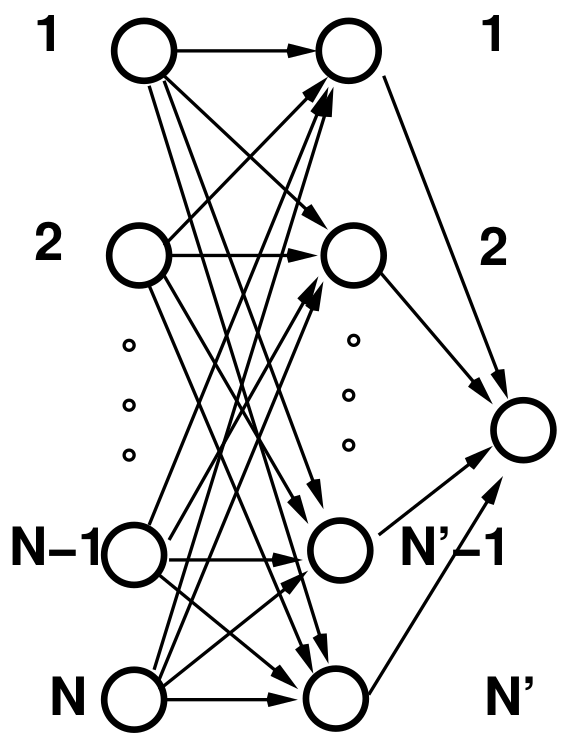
\includegraphics[width=0.3\textwidth]{Figuras/ejer_2_NN1.png}
    \caption{Esquema de la arquitectura utilizada para resolver el problema del XOR generalizado.}
    \label{02:fig:Arquitectura}
\end{figure}

En la Figura \ref{fig:2_Resultados} se observan los resultados obtenidos para la función de costo y \textit{accuracy} en cada uno de los casos. En caso de que $N'>N$, los resultados son similares a los del ejercicio anterior, ya que en una pequeña cantidad de épocas se obtiene un 100\% de precisión. La situación se vuelve mas problemática al disminuir $N'$, en donde se observa que para $N'=N=5$ el aprendizaje de la red nunca alcanza una precisión total e incluso no mejora de manera monótona conforme avanzan las épocas. Los resultados son incluso peores cuando $N'<N$, en donde se requieren muchas mas épocas para que la red aprenda e incluso para $N'=1$ nunca se logra alcanzar un valor de \textit{accuracy} no nulo. Este problema es esperable, ya que el valor de $N'$ determina las dimensiones de las matrices de pesos de cada una de las capas. Al disminuir $N'$, menor sera la cantidad de componentes de estas matrices, con lo cual deberá ajustar una gran cantidad de datos de entrada ($2^{N}$) con menos grados de libertad, que, en caso de ser demasiado pocos, se presentara un problema de underfitting y la red no mejorara sus resultados.


\begin{figure}[h!]
    \centering
    \begin{subfigure}[h]{0.49\textwidth} 
        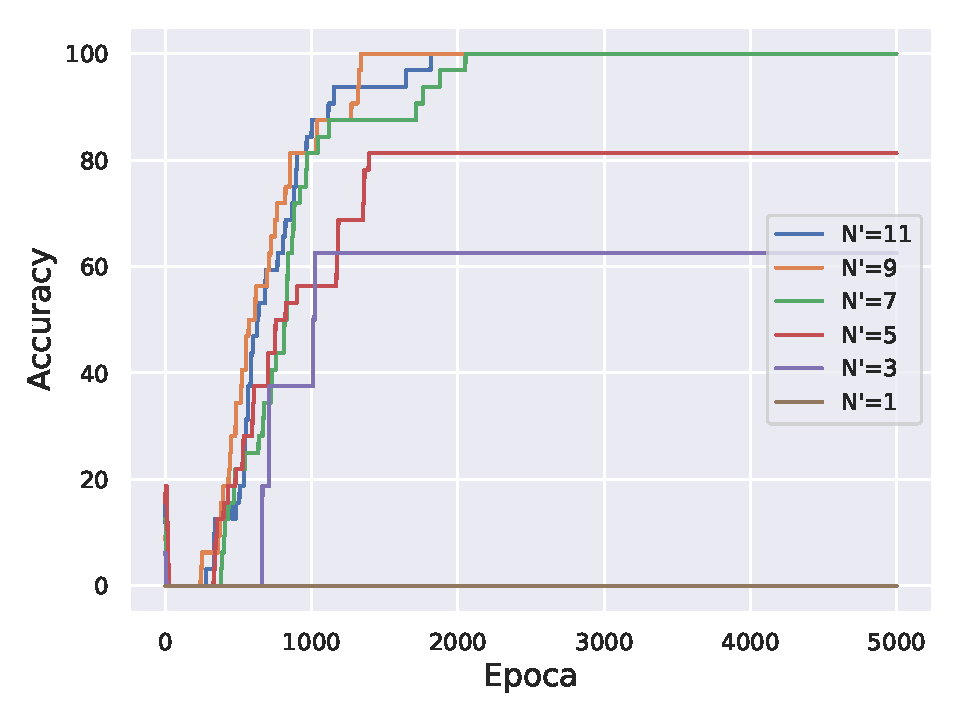
\includegraphics[width=\textwidth]{Figuras/ej2/Acc.pdf}
    \end{subfigure}       
    \begin{subfigure}[h]{0.49\textwidth} 
        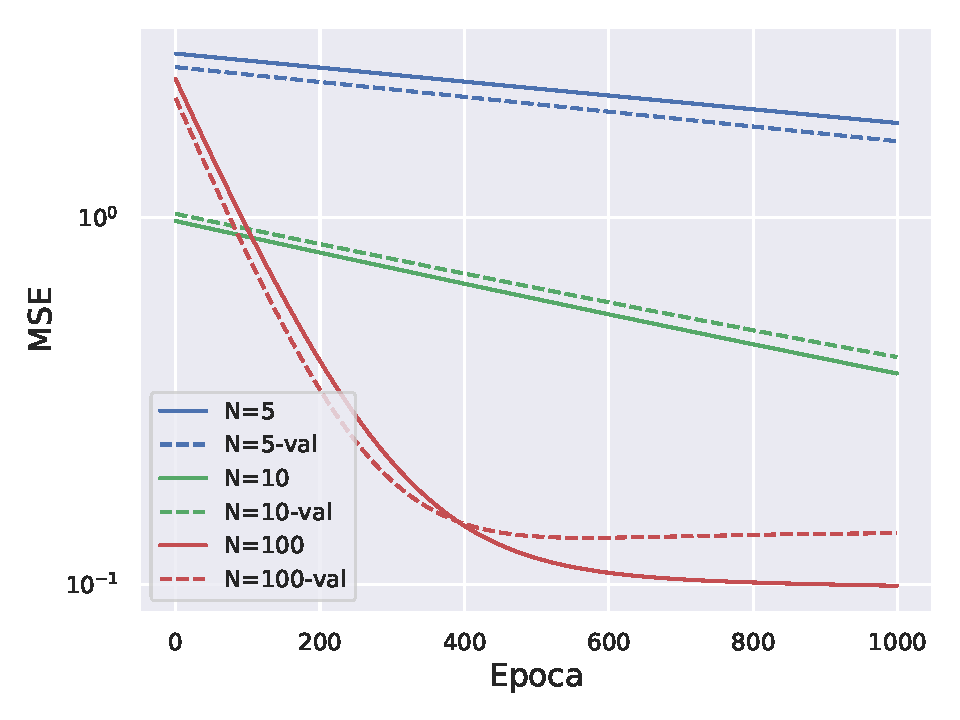
\includegraphics[width=\textwidth]{Figuras/ej2/Loss.pdf}
    \end{subfigure}
    \caption{Función de costo MSE y \textit{accuracy} para el entrenamiento de 6 modelos independientes variando la cantidad de neuronas de la capa oculta, utilizando la arquitectura propuesta en Fig. \ref{fig:1_Arquitecturas}.}
    \label{fig:2_Resultados}
\end{figure}


\bibliographystyle{acm}
\bibliography{biblio}

\end{document}



